\documentclass[10pt]{article}
\usepackage{amsmath}
\usepackage{commath}
\usepackage{algorithm}
\usepackage{algorithmic}
\usepackage{url}
\usepackage{cite}
\usepackage{amsfonts}
\usepackage{enumitem}
\usepackage{todonotes}
\usepackage{graphicx}
\graphicspath{{./images/}}

\begin{document}

\title{Applied and Computational Mathematics Master's Thesis Semester Report}
\author{Erick Galinkin}
\maketitle

\section{Introduction}
Malicious software (malware), has long been a burden on users of computers and of  the internet.
For individuals, a malware attack can cause the loss of their personal data and may allow hackers to access their bank accounts, steal their identity, or hold all of the files on their computer ransom.
The effects for a business can be particularly dire, with average cost of a malware attack sitting at \$1.7 million~\cite{seals2019threatlist}.
This problem is continuing to grow, and malware authors innovate in an effort to circumvent existing mitigating controls.

In the case of mobile malware, we often do not have the luxury of running computationally intensive processes on an endpoint and often cannot restrict devices that are brought into our environment.
 Traditional intrusion detection systems like Snort continue to mitigate known threats, but these signature-based systems suffer from the curse of reactivity for unknown threats.
 In order to mitigate these threats, controls must be generic enough to block threats which are unknown over any channel.

Our key contribution is an analysis of the impact Fourier and wavelet transforms have on unprocessed data as it relates to neural networks. 
This is achieved through an analysis of the efficiency and accuracy of a neural network that can detect the presence of malware on a mobile device without the need for an agent on the endpoint.
We compare this to a baseline random forest result and seek to explain what the network has learned and why different networks performance varies.

At the present time, the results may be divided into two categories:
\begin{enumerate}
\item Results on the augmented data associated with Watkins \textit{et al.}~\cite{watkins2018network} which suggest that a decision tree or other statistical learning method may be superior to a neural network and are explained below in section \ref{malware classifier}.
\item Analysis of how the representation of the data impacts the accuracy of a neural network and are explained in section \ref{data representation}
\end{enumerate}

\section{Previous Research}
The most significantly related previous research was conducted by Watkins \textit{et al.}~\cite{watkins2018network}.
This research yielded detections of mobile malware as the result of ping delays caused by CPU throttling in Android phones and an augmented version of their data set forms the basis for our research.
In the Watkins literature, a decision tree algorithm within the WEKA package was used to classify the traffic.
Similarly, we use a random forest from the Scikit-learn~\cite{scikit-learn} Python package as a baseline model.

Deep neural networks have been applied to related problems in information security, particularly detecting malicious executables on endpoints~\cite{raff2018malware} using techniques from natural language processing.
This research, conducted at Nvidia labs worked well at the endpoint, examining static properties of malicious and benign executables to draw determinations about the software from byte sequences.
Additionally, the strength of transfer learning in this domain has been observed in similar cases~\cite{galinkin2019shape} where convolutional neural networks were used to detect malicious code compiled for different architectures.
This suggests that byte sequence analysis may also be promising for convicting malicious network traffic.

words words words \todo{Put actual words here}

\section{Data}
The data were collected from 123 free Android apps downloaded from the Google Play store. 
Of these apps, 68 were benign and 55 were malicious.
The specific methods for collecting the data and classifying the samples is detailed in Watkins \textit{et al.}~\cite{watkins2018network}
Two datasets were examined for the classifier: these were ``request-reply'' data, and ``reply-reply'' data.
The request-reply data is the latency between a ping request being sent and a reply being received - 100 of these measurements were collected per sample.
The reply-reply data is quite similar except that the data measured the latency between a reply and a subsequent reply.

In addition to these two raw datasets, we also examined the Fourier transform of the datasets and a wavelet transform of the datasets. 
Given the large number of wavelets that exist, two different mother wavelets were considered: the Ricker wavelet and the Haar wavelet.
Summary statistics for these 8 datasets are in Table~\ref{Tab:summary}. 
For the non-raw datasets, only the first word of the transformed dataset is included (\textit{e.g.}, Fourier Transformed Request-Reply becomes ``Fourier Request'')

\begin{table}[]
\caption{Summary Statistics for Datasets}
\centering
\label{Tab:summary}	

\begin{tabular}{lllll}
\textbf{Dataset Name} & \textbf{Dataset Mean} & \textbf{Dataset Median} & \textbf{Mean Variance} & \textbf{Median Variance} \\
Request-Reply         & 27.43                 & 10.07                   & 8329.96                & 7663.89                  \\
Reply-Reply           & 98.52                 & 100.93                  & 2688.85                & 2465.29                  \\
Fourier Request       & 58.60*                & -1.45                   & 12229005.34            & 7418186.12               \\
Fourier Reply         & 100.19*               & -6.82                   & 119373138.03           & 122613924.30             \\
Wavelet Request       & 1.30                  & -.072                   & 1887.5                 & 1507.16                  \\
Wavelet Reply         & 1.03                  & 0.12                    & 2224.56                & 2135.86                 
\end{tabular}
\end{table}

\subsection{Analysis}
aaaa

\section{Models}
The neural networks were written in Python\footnote{Code is available at the following url: \url{https://github.com/erickgalinkin/jhu_masters}}, using the Tensorflow 2.0, PyTorch, and Scikit-learn libraries.
Only the baseline models described in \ref{other models} used the Scikit-learn library, and only the Wavelet Convolutional network described in \ref{wavelet cnn} used PyTorch.
The remaining models all used the Tensorflow framework.
All models were trained and tested on a 2018 MacBook Pro with 32GB of RAM and a 2.9GHz Intel Core i9 processor.
Given the small size of the data and relative simplicity of the models, GPU acceleration was not needed.

\subsection{Standard Fully-Connected Neural Network}
The fully-connected neural network architecture accepts, as input, a 1x100 row-vector. 
This vector is then fed to three densely connected layers, each with 256 ReLU-activated neurons.
The output neuron is a single sigmoid-activated neuron, which provides a probability of traffic being benign.

\subsection{Standard Convolutional Neural Network}
Our standard convolutional neural network is a sequential model which accepts the same sort of input as our fully-connected neural network, and passes it to an architecture comprised of two convolution and max-pooling blocks, followed by batch normalization, and then passed to two densely connected layers of 128 neurons each. The architecture is visualized below in figure \ref{fig:conv net}.

\begin{figure}[h]
\caption{Standard Convolutional Neural Network Architecture}
\label{fig:conv net}
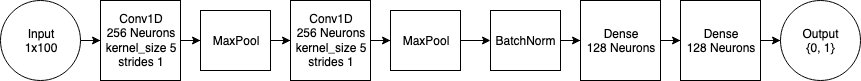
\includegraphics[width=\textwidth]{conv_architecture}
\centering
\end{figure}

\subsection{Fourier Convolutional Neural Network}
The Fourier Convolutional Neural Network leverages a custom "Fourier Layer", which moves the data into Fourier space via the Fast Fourier Transform before it performs a dot product on the input to the neuron.
Specifically, given an input $X^{(n)}$ and an output $A$, where the superscript is not an exponent, but instead indicates the layer of the input, the Fourier layer, $\ell$ acts on $X$: 
\begin{align*}
X^{(n+1)} & = a \\
& = \ell^{(n)}(X^{(n)}) \\
& = \sigma(\mathcal{F}^{-1}(\mathcal{F}(X^{(n)})\cdot \mathbf{W}^{(n)\top}))
\end{align*}

Where $\mathcal{F}$ is the Fast Fourier Transform, $\sigma$ is the activation function - ReLU in this case - and $\mathbf{W}$ is the weight matrix for layer n.

\begin{algorithm}
\caption{Fourier Layer}
\label{Fourier layer}
\begin{algorithmic}[1]
\REQUIRE $X, W \in \mathbb{C}^{mxn}, \beta \in \mathbb{C}^m$
\ENSURE $X \neq 0$
\STATE Perform Fourier transform on input data: $\mathcal{F}(X^{(n)})$
\STATE Take dot product of input data and weight matrix: $\mathcal{F}(X^{(n)})\cdot \mathbf{W}^{(n)\top}$
\STATE Perform Inverse Fourier transform on the dot product: $\mathcal{F}(\mathcal{F}(X^{(n)})\cdot \mathbf{W}^{(n)\top})$
\STATE Apply ReLU activation: $a = \sigma(\mathcal{F}^{-1}(\mathcal{F}(X^{(n)})\cdot \mathbf{W}^{(n)\top}))$
\STATE Return $a$
\end{algorithmic}
\end{algorithm}

Our Fourier ``Convolutional'' neural network - it is effectively a convolution, but no actual convolution operation occurs - is a mirror image of our standard convolutional neural network, only with the convolutional layers replaced by Fourier layers. 

\subsection{Wavelet Convolutional Neural Network} \label{wavelet cnn}
aaaa

\subsection{Other Models} \label{other models}
aaaa

\section{Results}
aaaa

\subsection{Malware Classifier} \label{malware classifier}
aaaa

\subsection{Data Representation and Neural Networks} \label{data representation}
aaaa

\section{Ongoing Work}
Based on the difficulty and apparent inefficiency on small datasets of the Fourier and Wavelet neural networks, alternate activation functions were considered. 
However, finding good spectral activation functions is still an open research question.
Pennec and Arsigny~\cite{pennec2013information} suggest that in high dimensional spaces, we can view our data as a manifold and thereby consider the Riemannian center of mass or \textit{Frechet mean} of the manifold.
Further research by Chakraborty \textit{et al.}~\cite{chakraborty2019surreal} suggests that in manifold-valued data, the possibility of using the tangent-ReLU activation function may make it feasible to move the data to and from the Fourier domain only once per pass through the network, instead of once per layer.
At this point, none of these techniques have been implemented in code, and our data may be too simple to fully validate the efficacy of these techniques.

\section{Conclusion}
aaaa

\bibliography{bibtex}
\bibliographystyle{siam}

\end{document}
